\begin{tikzpicture}[scale=0.95, every node/.style={font=\small}]
    \initialstate{q0}{(0,0)}{$q_0$}{(-1.0,0)}{west}
    \state{q1}{(2.0,0)}{$q_1$}
    \acceptingstate{q2}{(4.0,0)}{$q_2$}

    \transitionarrow[loop above]{q0}{above}{$b$}{q0}
    \transitionarrow[bend left=15]{q0}{above}{$a$}{q1}

    \transitionarrow[loop above]{q1}{above}{$a$}{q1}
    \transitionarrow[bend left=15]{q1}{above}{$b$}{q2}

    \transitionarrow[bend left=20]{q2}{below}{$a$}{q1}
    \transitionarrow[bend left=50]{q2}{above}{$b$}{q0}
\end{tikzpicture}
